\documentclass{article}
\usepackage{graphicx}

\title{Discovering Artificial Neural Networks with Perceptrons}
\author{Ludovic DEBEVER}
\date{May 2024}

\begin{document}

\maketitle

 
\begin{figure}[!h]
    \centering
    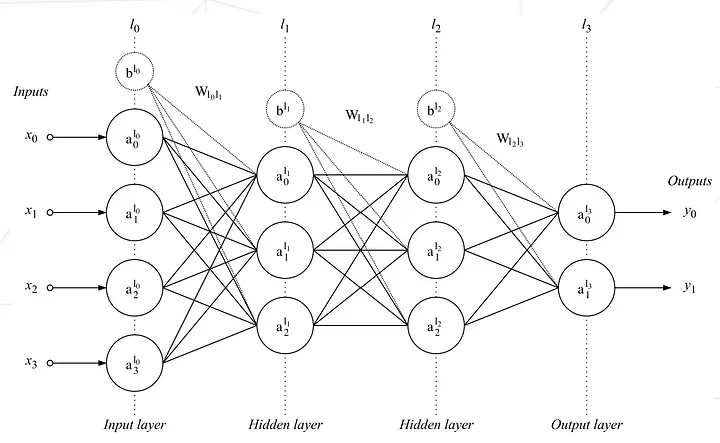
\includegraphics[width=1\linewidth]{assets/cover.png}
    \label{fig:cover}
\end{figure}

\newpage

\section{Introduction}

The rise of Artificial Intelligence has had a huge impact on most domains related to Information Technology. Developers, Writers, Designers, and others have been empowered by these new solutions, which have transformed the way tasks are approached and executed, leading to increased efficiency, creativity, and innovation across various fields. These advancements have facilitated the automation of repetitive tasks, enhanced decision-making processes, and enabled the creation of more sophisticated and personalized user experiences.

In this paper, we will explore how Artificial Intelligence can help Doctors classify diseases such as pneumonia using chest X-ray scans. By leveraging machine learning algorithms and deep neural networks, AI systems can analyze medical images with remarkable accuracy and speed, assisting healthcare professionals in diagnosing conditions more effectively. We will delve into the technical aspects of these AI models, examining their training processes, the data sets used, and the techniques employed to ensure reliability and precision.

\begin{figure}[!htb]
\minipage{0.32\textwidth}
  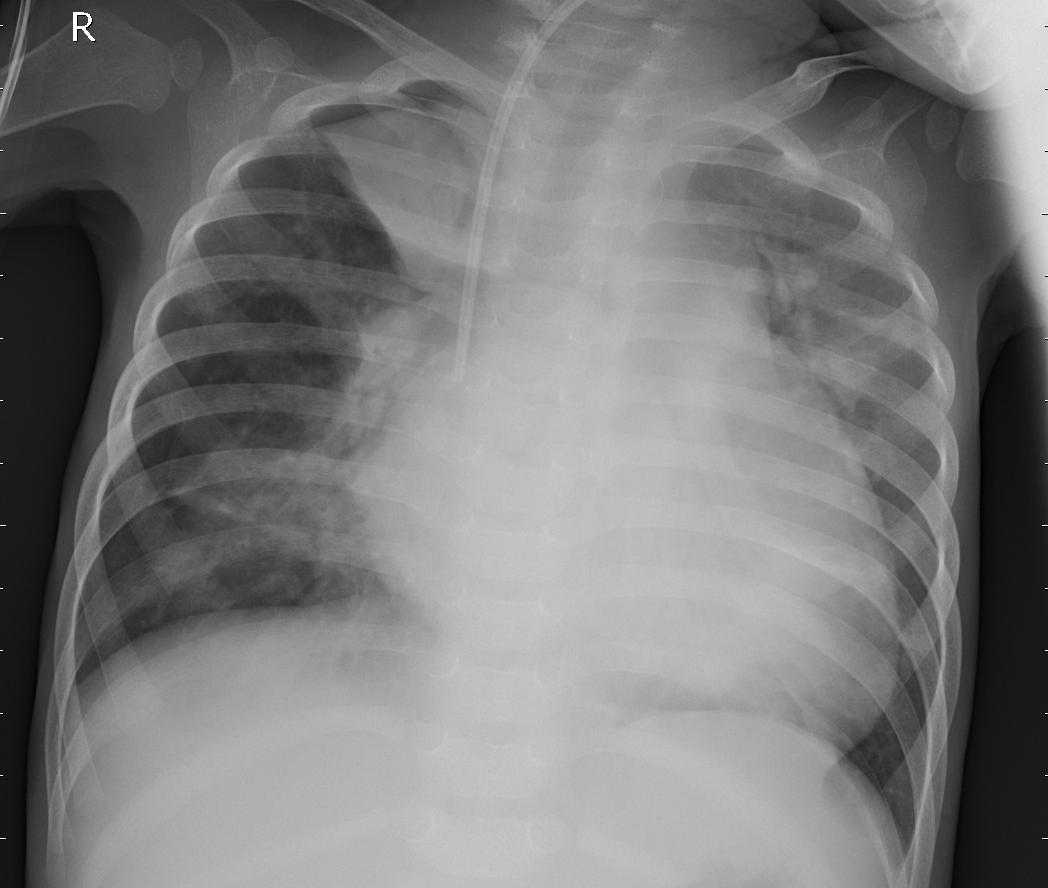
\includegraphics[width=\linewidth]{assets/intro/scan-bacteria.jpeg}
  \caption{Bacteria}\label{fig:scan-bacteria}
\endminipage\hfill
\minipage{0.32\textwidth}
  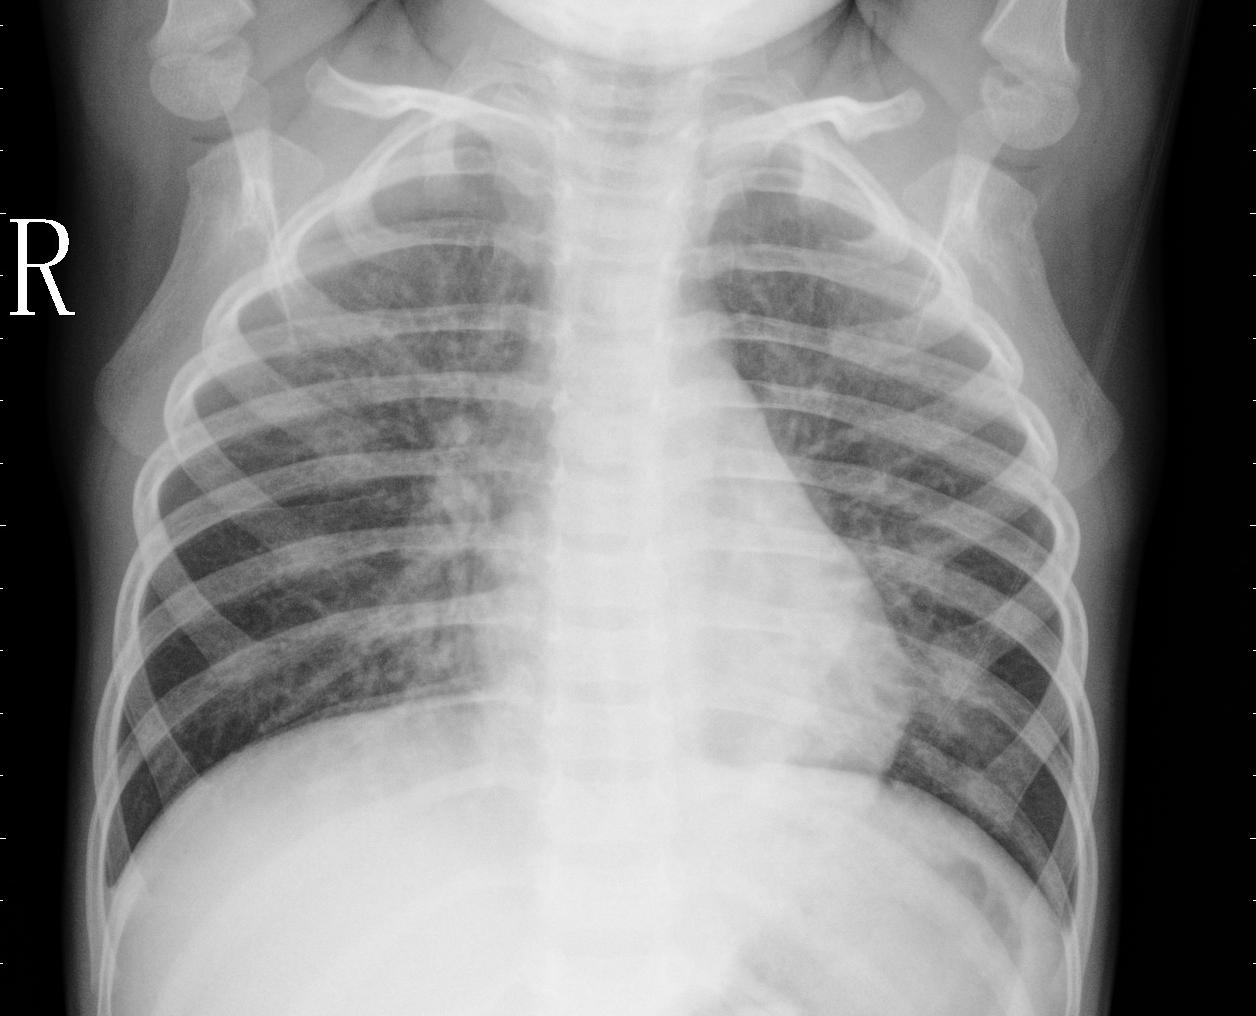
\includegraphics[width=\linewidth]{assets/intro/scan-virus.jpeg}
  \caption{Virus}\label{fig:scan-virus}
\endminipage\hfill
\minipage{0.32\textwidth}%
  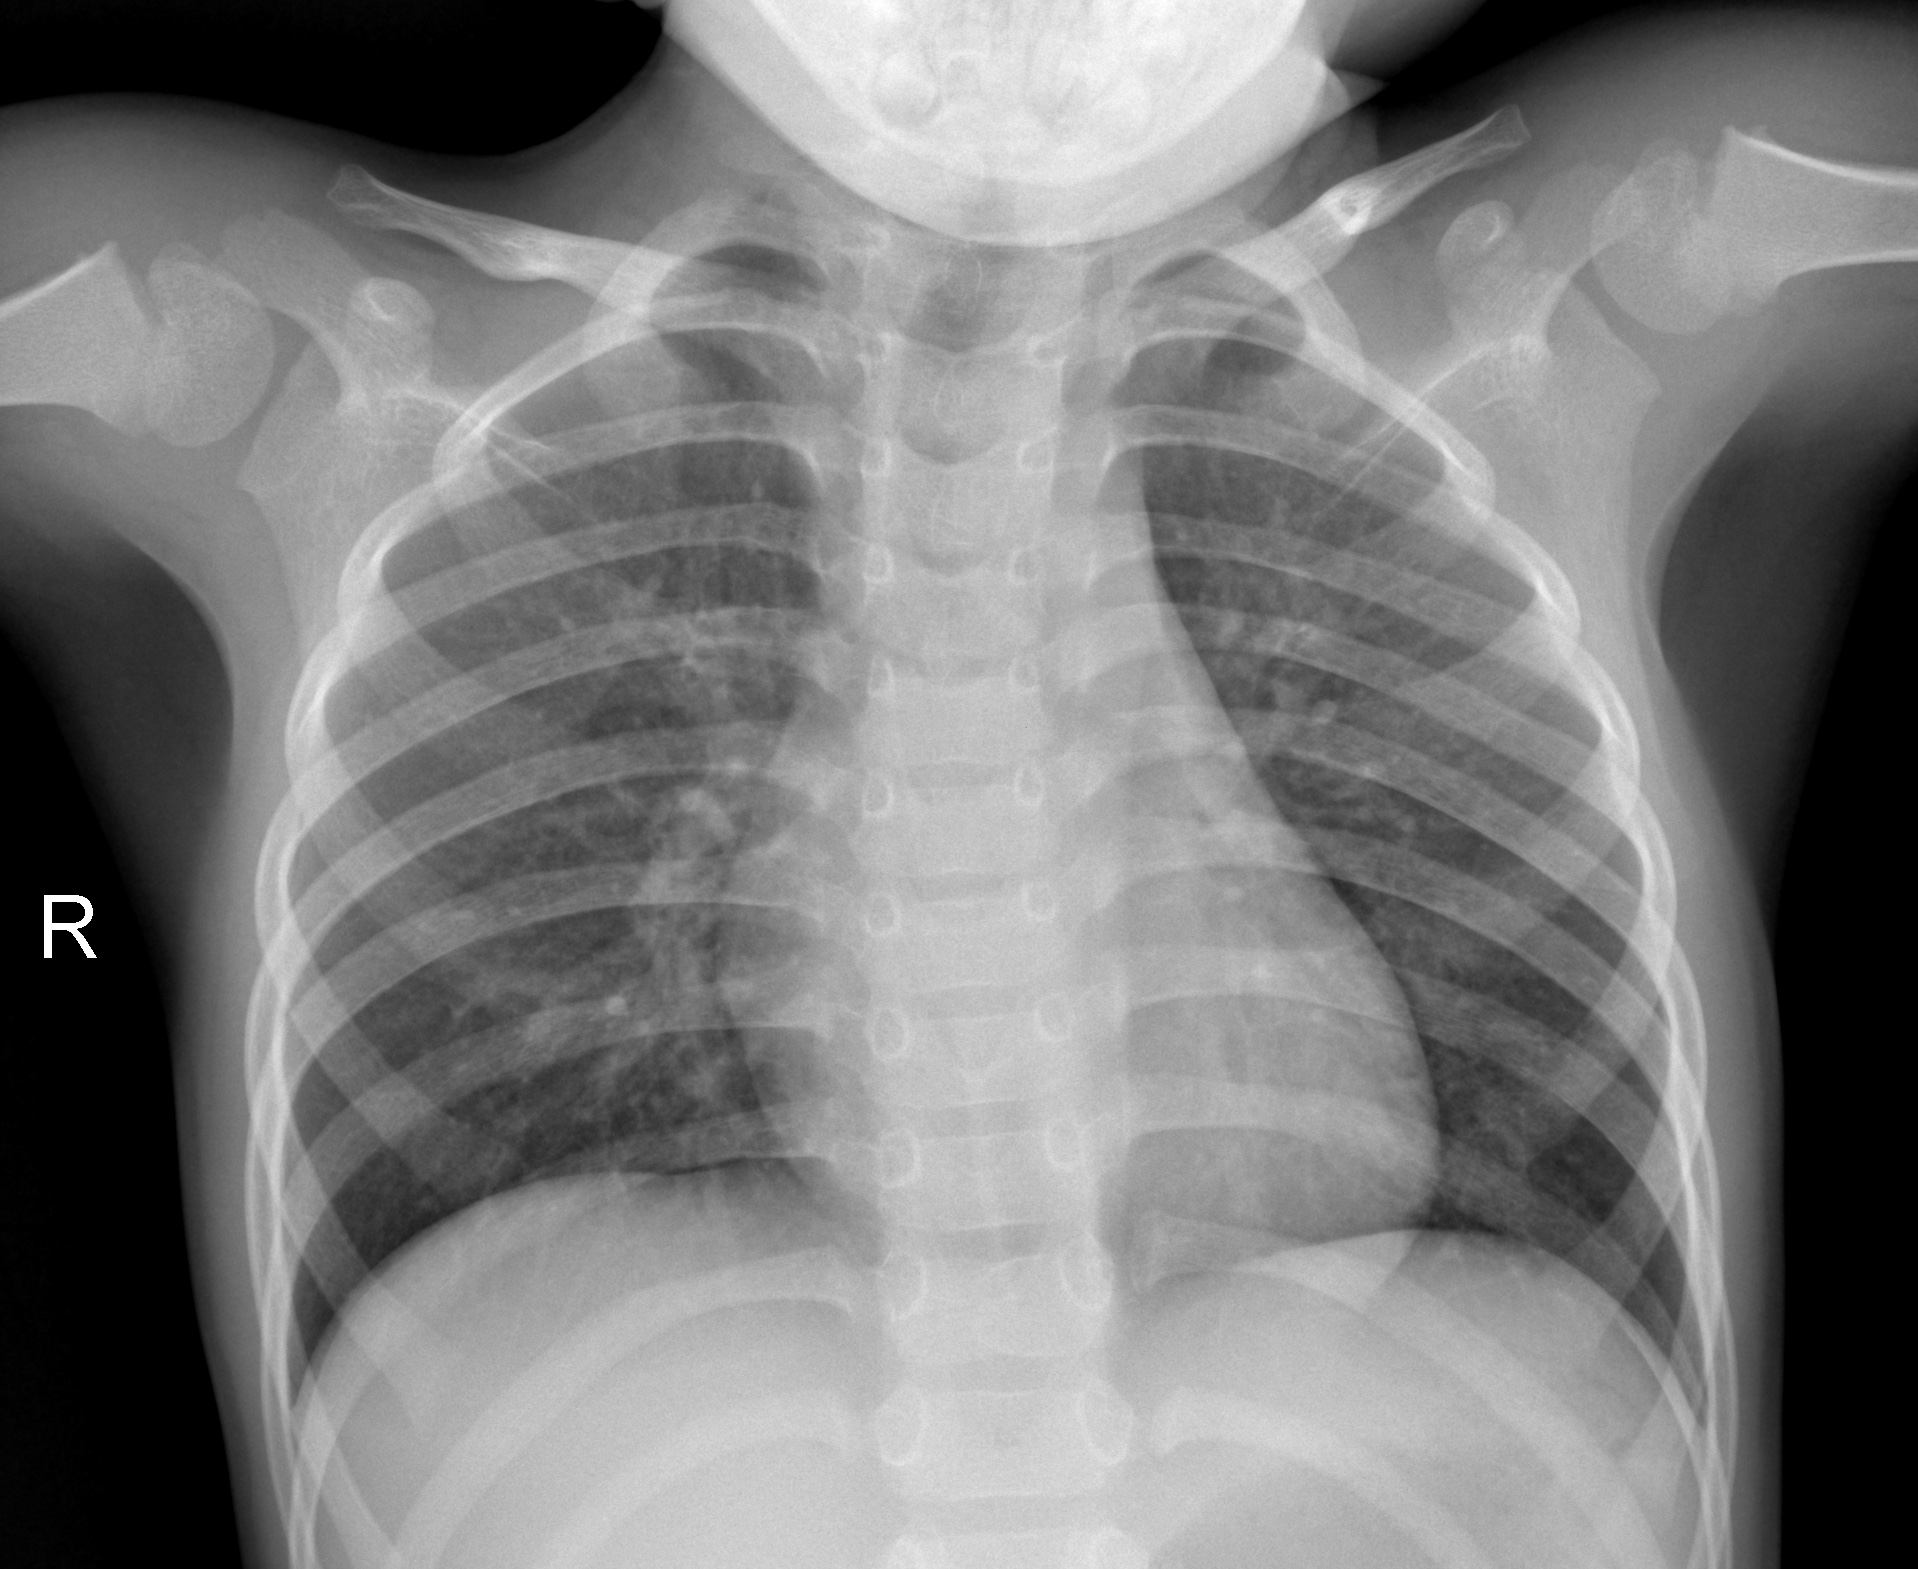
\includegraphics[width=\linewidth]{assets/intro/scan-normal.jpeg}
  \caption{Normal}\label{fig:scan-normal}
\endminipage
\end{figure}

\section{Frank Rosenblatt's Perceptron}

In 1957, Frank Rosenblatt invented the Perceptron, the simplest form of neural network and one of the first models to demonstrate machine learning. This groundbreaking model laid the foundation for future advancements in the field, as it was one of the earliest systems capable of learning from data. A model that would later be applied to fields such as image processing and speech recognition, it showcased the potential of machine learning to tackle complex tasks by improving performance through experience.

Based on a simple algorithm, the Perceptron could adapt to the input data in order to perform better over time. However, despite its innovative approach, the Perceptron had hard limitations. It could not solve non-linear problems, meaning it struggled with tasks where the relationship between input and output was not straightforward. This limitation was famously highlighted by Marvin Minsky and Seymour Papert in their 1969 book "Perceptrons," which demonstrated that the Perceptron could not handle the XOR problem, a simple example of a non-linear classification task.

\subsection{How does a Perceptron learn?}

The Perceptron involves principles that are foundational to modern artificial intelligence. It comprises key components such as Inputs and Weights, an Activation Function, and Back-propagation. At its core, the Perceptron is a single neuron directly connected to the inputs. Each input is assigned a specific weight, which represents its importance in the prediction process. To make a prediction, the Perceptron calculates the weighted sum of all inputs, which is the sum of each input multiplied by its corresponding weight.

Once the weighted sum is computed, the Perceptron employs an activation function to determine the output. In this simplified model, we use a threshold as the activation function. If the weighted sum exceeds the set threshold, the Perceptron produces a positive result; otherwise, it returns a negative result. This binary classification process allows the Perceptron to distinguish between two classes based on the input data.

\begin{figure}[ht]
    \caption{Perceptron}
    \centering
    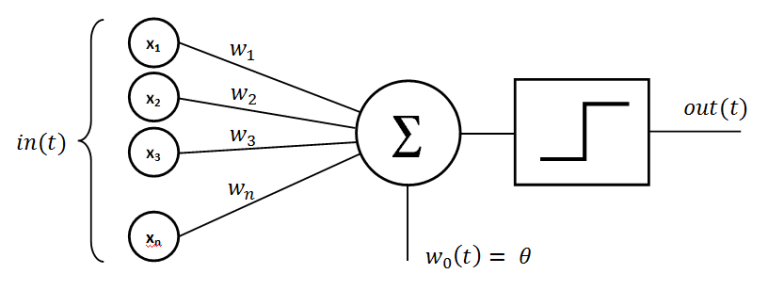
\includegraphics[width=0.75\linewidth]{assets/perceptron/perceptron.png}
    \label{fig:perceptron}
\end{figure}

To improve its performance over time, the Perceptron uses a learning process called Back-propagation. During training, the Perceptron adjusts its weights based on the errors between the predicted and actual outcomes. By iteratively updating the weights to minimize these errors, the Perceptron learns to make more accurate predictions.

\subsection{Classifying Images using the Perceptron}

Using the model we discussed earlier, we can classify images. However, due to the Boolean nature of the Perceptron's output, it can only differentiate between two classes. Before we proceed, we need to normalize our data. Each image will be resized to a fixed number of pixels—50x50 in this case—which provides a good balance between detail and low memory usage. Then, the color ranges will be converted to gray-scale values, leaving us with a single number per pixel. Each of these gray-scale values will serve as an input to the Perceptron. The final step before starting the training process is to define the hyper-parameters, which are the human-controlled settings of the model. For a Perceptron, these include the learning rate, the activation function, the number of epochs, and the number of inputs. We will use a simple threshold for the activation function, and the number of inputs has already been established during data normalization. Therefore, we only need to define the learning rate. The learning rate is crucial during the Perceptron's learning phase; after predicting a value and calculating the error, the error is multiplied by the learning rate and used to adjust the weights accordingly. There is no perfect value for the learning rate, but it needs to be small enough to allow the back-propagation process to find precise values for the Perceptron's weights.

\begin{figure}[ht]
    \centering
    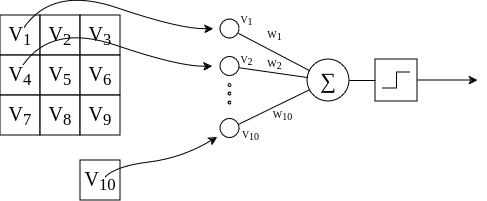
\includegraphics[width=0.75\linewidth]{assets/intro/perceptron-image-classification.png}
    \caption{Image Classification Perceptron}
    \label{fig:perceptron-image-classification}
\end{figure}

\end{document}
